\documentclass{article}%
\usepackage[T2A,T1]{fontenc}%
\usepackage[utf8]{inputenc}%
\usepackage{geometry}%
\geometry{tmargin=20mm,bmargin=20mm,lmargin=20mm,rmargin=20mm}%
\usepackage{newtxtext, newtxmath}%
\usepackage{substitutefont}%
\usepackage{lastpage}%
\usepackage{gensymb}%
\usepackage{ragged2e}%
\usepackage{graphicx}%
\usepackage{amsmath}%
\usepackage{subcaption}%
\usepackage{enumitem}%
\usepackage{fancyhdr}%
%
\linespread{1.5}%
\usepackage{newunicodechar}%
\fancypagestyle{header}{%
\renewcommand{\headrulewidth}{0.5pt}%
\renewcommand{\footrulewidth}{1.0pt}%
\fancyhead{%
}%
\fancyfoot{%
}%
\fancyhead[C]{%
TECHNICAL SCOPE OF WORK: PHASE 1 EARTHWORKS AND CIVILS%
}%
\fancyfoot[L]{%
H{-}MAC539{-}RFT{-}OE{-}0331{-}001{-}SHT{-}001%
}%
\fancyfoot[R]{%
Page \thepage\ of \pageref{LastPage}%
}%
}%
%
\begin{document}%
\pagestyle{empty}%
\normalsize%
\pagestyle{header}%
\begin{center}%
\section*{}%
\label{sec:}%
\begin{minipage}{\textwidth}%
\centering%
\begin{Large}%
\textbf{MAC MINING AND CONSTRUCTION PARTNERS LIMITED}%
\end{Large}%
\vspace*{20pt}%
\linebreak%
\begin{large}%
\textbf{RIVER WATER ABSTRACTION}%
\end{large}%
\vspace*{20pt}%
\linebreak%
\begin{large}%
\textbf{H{-}MAC539}%
\end{large}%
\vspace*{20pt}%
\linebreak%
\begin{large}%
\textbf{H{-}MAC539{-}RFT{-}OE{-}0331{-}001{-}SHT{-}001}%
\end{large}%
\vspace*{80pt}%
\end{minipage}

%
\end{center}%
\begin{center}%
\begin{minipage}{\textwidth}%
\flushleft%
\begin{tabular}{|l |l |}%
\hline%
\textbf{Engineer:}&Gerald Holt (Pr.Eng)\\%
\cline{1%
-%
2}%
\textbf{Registration:}&20020259\\%
\cline{1%
-%
2}%
\textbf{Email:}&gerald@macpartnersltd.com\\%
\cline{1%
-%
2}%
\textbf{Phone:}&+233{-}0254{-}1525\\%
\cline{1%
-%
2}%
\textbf{Adress:}&Plot 19A\\%
\cline{1%
-%
2}%
\textbf{}&Okpoti Street\\%
\cline{1%
-%
2}%
\textbf{}&Adenta, Accra, Ghana\\%
\cline{1%
-%
2}%
\textbf{Website:}&www.macpartnersltd.com\\%
\cline{1%
-%
2}%
\end{tabular}%
\vspace*{150pt}%
\centering%
\end{minipage}%
\end{center}%


\begin{figure}[h!]%

\includegraphics[width=240px]{C:/_EEMS/apps/accounts/logos/MAC.jpg}%
\centering%
\end{figure}

%
\newpage%
\begin{center}%
\section*{REVISION HISTORY}%
\label{sec:REVISIONHISTORY}%

%
\begin{minipage}{\textwidth}%
\centering%
\begin{tabular}{|c |c |c |c |c |c |}%
\hline%
\textbf{REV}&\textbf{DESCRIPTION}&\textbf{DATE}&\textbf{ISSUED BY}&\textbf{REVIEWED BY}&\textbf{APPROVED}\\%
\hline%
A&ISSUED FOR REVIEW&2022{-}10{-}12&G.G. HOLT&H.F. HOLT&\\%
\hline%
B&ISSUED FOR REVIEW&2022{-}10{-}14&G.G. HOLT&H.F. HOLT&\\%
\hline%
\end{tabular}%
\end{minipage}%
\end{center}%
\newpage%
\section{CUSTOMER DETAILS}%
\label{sec:CUSTOMERDETAILS}%
\begin{flushleft}%
\begin{minipage}{\textwidth}%
\centering%
\begin{tabular}{|l |l |}%
\hline%
\textbf{Customer:}&Cardinal Namdini Mining Ltd\\%
\cline{1%
-%
2}%
\textbf{Customer Name:}&Bright Dzah\\%
\cline{1%
-%
2}%
\textbf{Customer Email:}&bright.dzah@cardinalresources.com.au\\%
\cline{1%
-%
2}%
\end{tabular}%
\end{minipage}%
\end{flushleft}

%
\newpage%
\section{PROJECT DATA}%
\label{sec:PROJECTDATA}%
\subsection{Applicable Codes}%
\label{subsec:ApplicableCodes}%
\begin{flushleft}%
\begin{minipage}{\textwidth}%
\flushleft%
\begin{tabular}{|l |l |}%
\hline%
\textbf{SANS 10208:}&Design of structure for the mining industry Part 3: Conveyances\\%
\hline%
\textbf{SANS 10160:}&Buidling Loading Code\\%
\hline%
\textbf{SANS 10162:}&Steel Design Code\\%
\hline%
\textbf{SANS 10100{-}1:}&The Structural use of concrete Part 1 – Design\\%
\hline%
\textbf{SANS 10100{-}2:}&The Structural use of concrete Part 2 – Materials and Execution of Work\\%
\hline%
\textbf{SANS 10144:}&Detailing of steel reinforcement for concrete\\%
\hline%
\textbf{SANS 10161:}&The design of foundations for buildings\\%
\hline%
\textbf{SANS 110:}&Sealing components for the building industry, two components, polysulphide base\\%
\hline%
\textbf{SANS 10164:}&The structural use of masonry Part 1\\%
\hline%
\textbf{BS 2853:}&The design and testing of steel overhead one way beams\\%
\hline%
\textbf{AWS D1.1:}&Structural Welding Code {-} Steel\\%
\hline%
\textbf{SANS 10120{-}3:}&Corrosion protection systems for steelwork\\%
\hline%
\textbf{EN 10025:}&Hot rolled products of structural steel\\%
\hline%
\textbf{SANS 986:}&Pre{-}cast reinforced concrete culverts\\%
\hline%
\textbf{SANS 1077:}&Sealing compound for the building and construction industry, two components, polyurethane base\\%
\hline%
\textbf{BS 3148:}&Test for water for making concrete\\%
\hline%
\textbf{BS 5075{-}1:}&Concrete admixtures\\%
\hline%
\textbf{BS 5075{-}2:}&Specification for accelerating admixtures, retarding admixtures and water reducing admixtures\\%
\hline%
\textbf{BS 5075{-}3:}&Specification for air{-}entraining admixtures\\%
\hline%
\textbf{BS 5075{-}4:}&Specification for superplasticizing admixtures\\%
\hline%
\textbf{BS 5838:}&Specification for dry packed cementitious mixes\\%
\hline%
\textbf{BS 5838{-}1:}&Prepacked concrete mixes\\%
\hline%
\textbf{BS 5838{-}2:}&Prepacked mortar mixes\\%
\hline%
\end{tabular}%
\end{minipage}%
\end{flushleft}

%
\subsection{Site Conditions}%
\label{subsec:SiteConditions}%
\begin{flushleft}%
\begin{minipage}{\textwidth}%
\flushleft%
\begin{tabular}{|l |l |c|}%
\hline%
\textbf{Country}&Ghana&\\%
\hline%
\textbf{Region}&Talensi District (Upper East Region of Ghana)&\\%
\hline%
\textbf{Closest Regional Centre}&Bolgatanga&\\%
\hline%
\textbf{Distance to Regional Centre}&50&$km$\\%
\hline%
\textbf{Main Route to Regional Centre}&Talensi Trunk Road off the Tamale{-}Bolgatango Highway&\\%
\hline%
\textbf{Elevation Above Sea Level}&190&$m AMSL$\\%
\hline%
\textbf{Coordinates}&10.63 ° N (Latitude)&\\%
\hline%
\textbf{}&0.66 ° W (Longitude)&\\%
\hline%
\textbf{Area Climate}&Cool, Dry and Dusty&\\%
\hline%
\textbf{Maximum Temperature}&39.3&$°C$\\%
\hline%
\textbf{Average Temperatren}&28.9&$°C$\\%
\hline%
\textbf{Minimum Temperature}&19.3&$°C$\\%
\hline%
\textbf{Maximum Humidity}&68.8&$\%$\\%
\hline%
\textbf{Average Humidity}&46.5&$\%$\\%
\hline%
\textbf{Minimum Humidity}&40.3&$\%$\\%
\hline%
\textbf{Maximum Annual Rainfall}&1464&$mm/a$\\%
\hline%
\textbf{Average Annual Rainfall}&1022&$mm/a$\\%
\hline%
\textbf{Minimum Annual Rainfall}&May to October&\\%
\hline%
\textbf{Maximum Rainfall in 24 hours}&160&$mm$\\%
\hline%
\end{tabular}%
\end{minipage}%
\end{flushleft}

%
\newpage%
\subsection{Sketches and Drawings}%
\label{subsec:SketchesandDrawings}%
\subsubsection{Basic Flow Diagram}%
\label{ssubsec:BasicFlowDiagram}%


\begin{figure}[h!]%
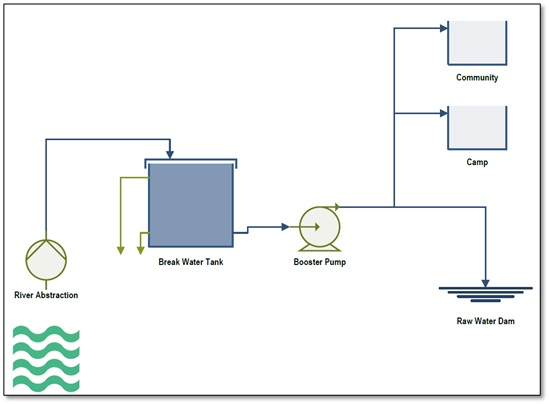
\includegraphics[width=450px]{C:/_EEMS/apps/documents/tenderSOW/images/BasicFlowChart.jpg}%
\centering%
\caption{Basic Flow Diagram}%
\centering%
\end{figure}

%
\subsubsection{General Layout}%
\label{ssubsec:GeneralLayout}%


\begin{figure}[h!]%
\begin{subfigure}[b]{0.45\linewidth}%
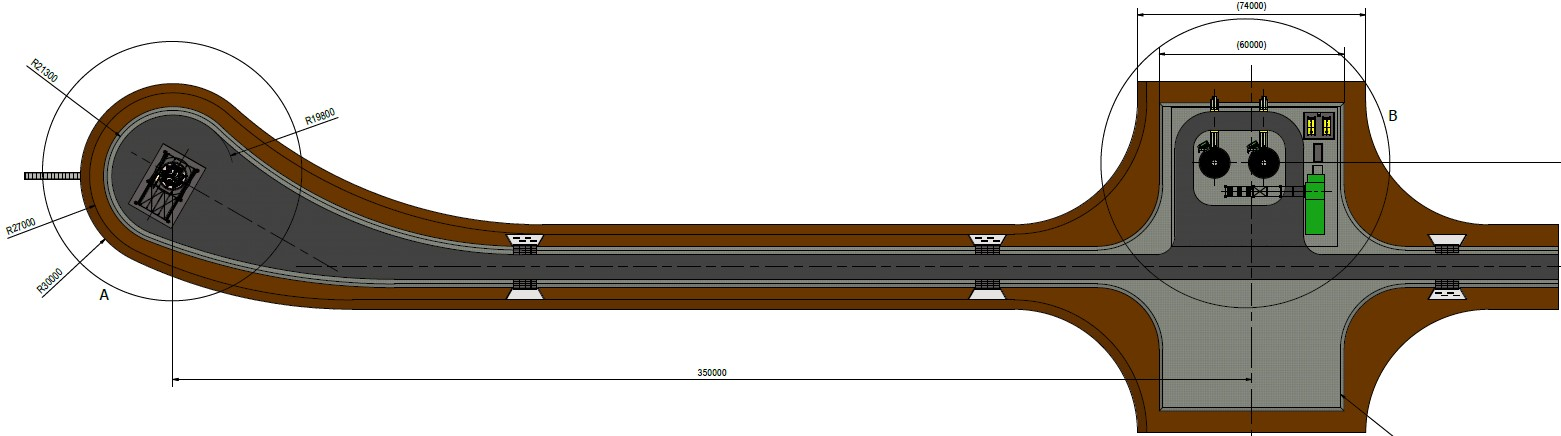
\includegraphics[width=500px]{C:/_EEMS/apps/documents/tenderSOW/images/OverallLayout.jpg}%
\centering%
\caption{Overall River Abstraction Layout}%
\end{subfigure}%
\end{figure}

%
\newpage

%
\subsubsection{River Abstraction Detail}%
\label{ssubsec:RiverAbstractionDetail}%


\begin{figure}[h!]%
\begin{subfigure}[b]{0.45\linewidth}%
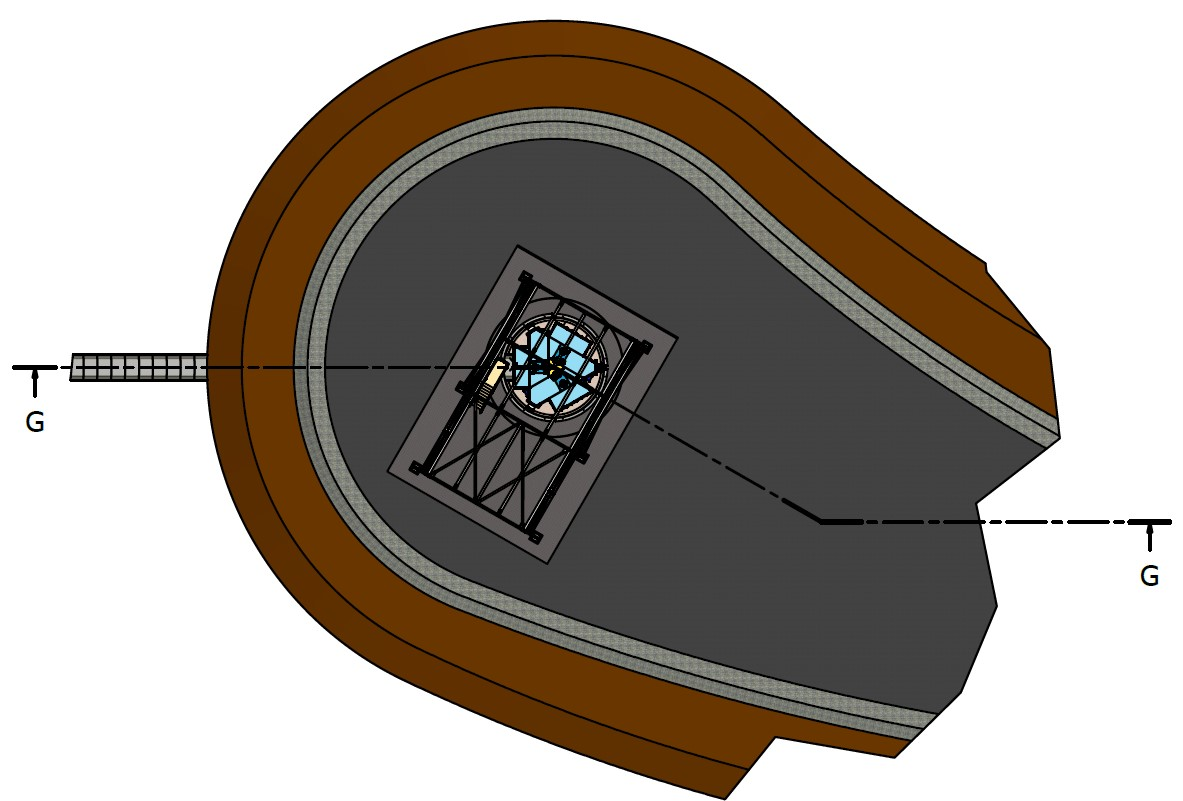
\includegraphics[width=500px]{C:/_EEMS/apps/documents/tenderSOW/images/RiverAbstract1.jpg}%
\centering%
\caption{River Abstraction Detail 1}%
\end{subfigure}%
\end{figure}

%


\begin{figure}[h!]%
\begin{subfigure}[b]{0.45\linewidth}%
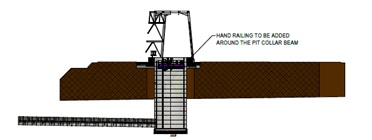
\includegraphics[width=500px]{C:/_EEMS/apps/documents/tenderSOW/images/RiverAbstract2.jpg}%
\centering%
\caption{River Abstraction Detail 2}%
\end{subfigure}%
\end{figure}

%


\begin{figure}[h!]%
\begin{subfigure}[b]{0.45\linewidth}%
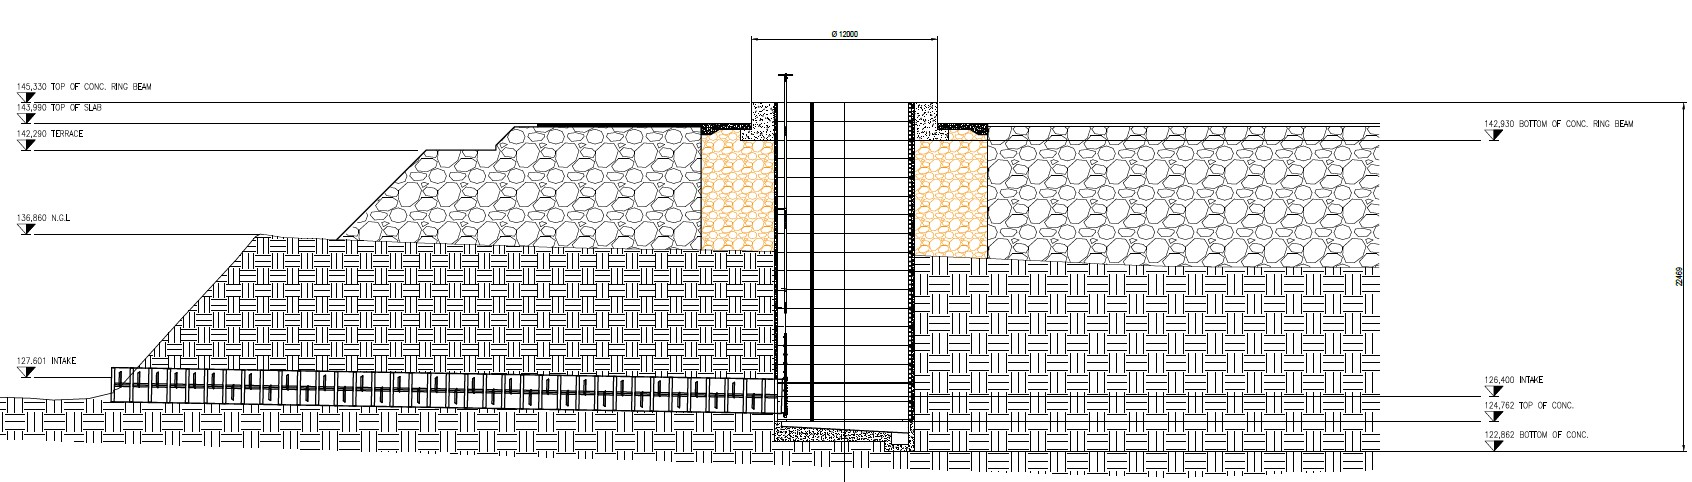
\includegraphics[width=560px]{C:/_EEMS/apps/documents/tenderSOW/images/RiverAbstract3.jpg}%
\centering%
\caption{River Abstraction Detail 3}%
\end{subfigure}%
\end{figure}

%


\begin{figure}[h!]%
\begin{subfigure}[b]{0.45\linewidth}%
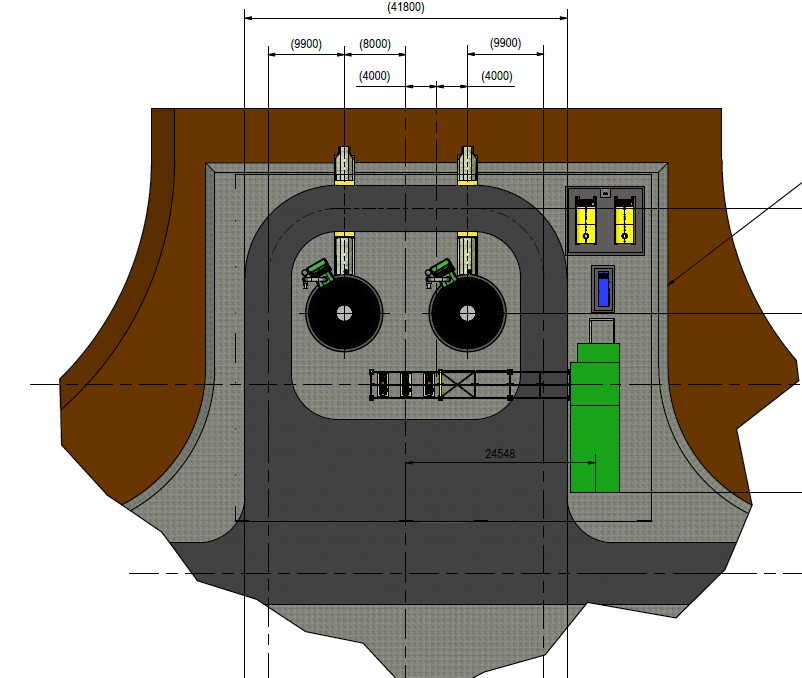
\includegraphics[width=500px]{C:/_EEMS/apps/documents/tenderSOW/images/Booster.jpg}%
\centering%
\caption{Booster Station}%
\end{subfigure}%
\end{figure}

%
\newpage%
\section{PROJECT INFORMATION}%
\label{sec:PROJECTINFORMATION}%
\subsection{Introduction}%
\label{subsec:Introduction}%
Namdini is approximately 50 km southeast of the regional town of Bolgatanga in Northern Ghana and around 60 km south of the Burkina Faso border (Figure 19). Namdini lies within the Nangodi Greenstone Belt, one of a series of southwest–northeast trending granite-greenstone belts which host significant gold mineralization in Ghana and Burkina Faso.
The Talensi district which was part of the Talensi-Nabdam district became a separate district in 2012, through Legislative Instrument LI 2110, with Tongo as the capital. The district, which is one of the thirteen Municipalities and Districts in the Upper East Region, is bordered to the north by the Bolgatanga Municipality, to the south by West and East Mamprusi Districts (both in the Northern Region), to the west by Kassena-Nankana District, and to the east by the Bawku West and Nabdam Districts. The district lies between latitude 10° 15' and 10° 60' North of the equator and longitude 0° 31' and 1° 05' West of the Greenwich Meridian and covers a land area of 838.4 km2 with a total population of 81,194, which constitutes 7.8% of the regional population. It is made up of 96 towns and villages with a settlement pattern which is predominantly rural.
The topographic relief within the project area is generally flat with gently undulating terrain, rising to the south where the area is overlain by sediments. Elevation varies from 175 to 250 meters above mean sea level (“AMSL”) with average elevation at approximately 190 m. Physiography is primarily savannah grassland characterized by short, scattered drought-resistant trees, scrub, and grass that is seasonally burned by bushfires or scorched by the sun during the long dry season.%
\newline%
%
\newline%
%
As part of the water requirements for the process plant, river water abstraction is one of the methods that will be used to supply water to the plant as well as for the camp and accommodation area. The point of abstraction has been identified which is 10,910 meters from the plant. 
Water will be abstracted by means of vertical spindle pumps, which will discharge into breakwater tanks of the booster station, 350 meters from the river in a northern direction. The booster station will accommodate the diesel generator, MCC, diesel storage, and the booster pumps which will transfer the water to the raw water storage. 
Except for areas above ground and the abstraction point, all the piping will be HDPE piping buried next to the main road to the process plant.  Piping passing underneath the main road will also be constructed from steel. The line will be equipped with valve boxes and vacuum breakers as well as the necessary scour points. Also, along the line, a T-off will be installed for the supply line to the camp.

%
\subsection{River Abstraction}%
\label{subsec:RiverAbstraction}%
The point of abstraction is provided by the client. The coordinates of the abstraction point are X=748698.3955, Y=1178401.56, Z= 144.569 (cartesian system). This position was selected as it is the highest point along the river. This is important to accommodate the river level fluctuations and to ensure that the abstraction system is able to perform under these different conditions.%
\newline%
%
\newline%
%
 The following are the attributes of the river abstraction configuration:%
\begin{itemize}%
\item%
The catchpit centre is 45 meters from the riverbank. This distance has been increased from 20 meters to 45 meters to allow space for the causeway, access turning radius and soil stability.%
\item%
The level of the slab around the catch pit is at 143,990 mASL. The top of the catch pit ring beam is 145,330 mASL.%
\item%
Once the abstraction pump chamber earth, civil, and mechanical works are completed, the embankment left in situ to river to be removed during low level conditions of river. The section of soil embankment to be removed after construction of pump chamber must be stabilized by gabions.%
\item%
The centre of the inlet of the water intake pipe is at level 127,600 mASL. Note that the intake slope has been changed to the opposite of that of the original conceptual design. The intake water pipe slopes at 1° downward to the bottom of the catch pit bottom. The centre of the pipe enters the pit at level 126,400 mASL.%
\item%
As the area between transfer pump station and river embankment will flood due to its low elevation, a causeway (complete with culverts to allow water flow) has been incorporated for access to abstraction pumps.%
\item%
The power supply to abstraction pumps to run on the causeway.%
\end{itemize}

%
\subsection{Booster Station}%
\label{subsec:BoosterStation}%
The point of abstraction is provided by the client. The coordinates of the abstraction point are X=748698.3955, Y=1178401.56, Z= 144.569 (cartesian system).%
\newline%
%
\newline%
%
The following are the attributes of the booster station configuration:%
\begin{itemize}%
\item%
The station consists of two areas. On the western side of the causeway is the booster station and on the earstern side the contractor's laydown area.%
\item%
The booster pump station will house the buffer tanks, booster pumps and substation.%
\item%
The area will also be equipped with a building consisting of a security office, control room, store room, workshop and the substation.%
\end{itemize}

%
\newpage%
\section{PHASE 1: SCOPE OF WORK}%
\label{sec:PHASE1SCOPEOFWORK}%
\subsection{Battery Limits}%
\label{subsec:BatteryLimits}%
This tender is for Phase 1 of the project. Phase 1 is the earthworks and civils works for the causeway and catchpit. It is important that these activities are completed before the end of January 2023 as this is the time when the river is the lowest. The low river level is crucial for the safe installation of the intake water pipe.%
\newline%
%
\newline%
%
The battery limits for Phase 1 are as follows:%
\begin{itemize}%
\item%
All earthworks and filling from the booster station to the river abstraction area.%
\item%
The excvation and installation of the steel sections for the catch pit.%
\item%
The excvation and installation of the water intake pipe and the final cut through the river bank.%
\end{itemize}

%
\subsection{Preceeding Work}%
\label{subsec:PreceedingWork}%
\subsubsection{Clearing and Grubbing}%
\label{ssubsec:ClearingandGrubbing}%
\begin{enumerate}[label=\alph*),start=1]%
\item%
Refer to the applicable drawings for the correct levels. It is crucial that these levels are maintained. No deviation is allowed unless approved by the engineer.%
\item%
Avoid damage to the Site and to existing facilities, trees, peat, and shrubs designated to remain.%
\item%
Protect benchmarks,  baseline  monuments,  property  corners,  and other temporary or permanent survey markers in the vicinity of the Work from destruction or disturbance.%
\item%
Within the area to be cleared, properly relocate survey markers that interfere with the Work, or witness the markers and then restore them after completing the Work.%
\item%
Before starting clearing operations, erect protective barriers around trees, shrubs, and other facilities designated to remain. Erect barriers at or outside of the tree or shrub drip line. Do not use the area within protective barriers for traffic, storage, or any other purpose. After clearing and grubbing work is complete, properly remove and dispose of protective barriers.%
\item%
Preliminary survey location of road, piping corridor, gathering station, and other facilities shall be done using Total Station tools.%
\item%
Surveying shall be started from recommended GPS benchmarks and one other reference benchmark. From these two benchmarks, activity shall be continued to surveying of road and corridor centerline with minimum two survey points at both ends for every centerline. After obtain two reference points, activity shall be continued to the cutting line and stake out works. Output of preliminary survey is a general situation and preliminary stake out for guidance on detail survey.%
\item%
Move existing or master of benchmarks to the project site and built{-}up the local benchmarks or benchmark monument permanently. Local benchmark will be checked periodically to ensure the accuracy of elevations and coordinates. Benchmarks shall be protected from object disturbances.%
\item%
At least one local benchmark monument shall be provided for a quadrant. Additional benchmark monument shall be provided if one monument is not adequate.%
\item%
Theodolite and leveling shall be employed in surveying coordinates and elevations. Closed{-}polygon per quadrant method shall be used in surveying coordinates.%
\item%
Distance of stake out shall be 50 m up to 100 m, identified by wooden dolken, and marked by red color for easy identification. Temporary or permanent marker shall be protected from destruction or disturbance.%
\item%
All instruments shall be calibrated before used.%
\item%
Clearing shall be done on all areas, which is included borrow pit, road, corridor, and gathering station before starting the filling work.%
\item%
Clearing includes removal and proper disposal of trees, bushes, stumps, rubbish, and other vegetation resting on or protruding through the ground surface area to be cleared, without removing its roots. Clearing shall be performed at all back fill area without geotextile on base.%
\item%
All garbage material shall be stored at adjacent or destination area and shall not be burned.%
\item%
Stripping at borrow pit area includes cutting of topsoil up to maximum 300MM depth. Topsoil shall be stored around borrow pit area.%
\item%
Grubbing includes removal and disposal of roots, stumps, bushes and other obstruction materials, which protruding through the ground surface. Grubbing may include cutting of topsoil up to 100mm depth if required. Grubbing shall be performed at strong surface only. Grubbing at peat area shall not be performed.%
\item%
Especially for gathering station \& other plant areas, depth of excavation shall follow the approval engineering drawing.%
\item%
Trees with minimum 100mm diameter shall be selected from disposal materials and shall be used as corduroy material. These selected trees shall be stored in dry area before the installation.%
\item%
Other disposal materials such as topsoil, debris, and roots shall be spread around the location without disposing them outside the project area. This location shall be replanted.%
\item%
After clearing and grubbing have been completed, eliminate stump holes, depressions, ridges, and other irregular surface features by grading and backfilling to achieve a surface suitable for subsequent construction operations. Shape the resulting surface for positive drainage of surface runoff.%
\end{enumerate}

%
\subsubsection{Topsoil Removal and Stockpiling}%
\label{ssubsec:TopsoilRemovalandStockpiling}%
\begin{enumerate}[label=\alph*),start=1]%
\item%
Topsoil is generally representative of agriculturally productive  soil. Topsoil shall be free from subsoil and objectionable material that would hinder plant growth or maintenance and shall not contain more than 5\% by volume of stones larger than 25mm.%
\item%
Remove materials only to such depth that it meets the definition of topsoil. Strip and stockpile removed topsoil in areas to be excavated separately from other excavated materials. Protect topsoil stockpiles from contamination during progress of the work until their materials have been used in finish operations. Conserve acceptable topsoil from the Site sufficiently to cover areas requiring planting.%
\end{enumerate}

%
\subsection{Preparation}%
\label{subsec:Preparation}%
\subsubsection{Preliminary Site Examination}%
\label{ssubsec:PreliminarySiteExamination}%
\begin{enumerate}[label=\alph*),start=1]%
\item%
Prior the excavation, thoroughly examine the area to be excavated to verify the locations of features indicated on the drawings and to ascertain the existence and location of any underground structure or other item not shown that might interfere with the new structure or pipe installation. To notify COMPANY of any obstructions that will prevent accomplishment of the Work. Take protective measurement to prevent existing facilities within the work area that are not designated to be removed from being damaged by the Work.%
\end{enumerate}

%
\subsubsection{Fills and Embankments}%
\label{ssubsec:FillsandEmbankments}%
\begin{enumerate}[label=\alph*),start=1]%
\item%
Where the structure or pipeline is to be installed in an area of fill or embankment, verify that such work has been completed to an elevation at least 600mm above the bottom of the structure to be installed or at least 900mm above the top of the pipeline to be installed. No concrete base/slabs and trenches shall be placed on area of fill or embankment when the settlement processes still exist unless they are adequately supported on piles.%
\end{enumerate}

%
\subsubsection{Fills and Embankments}%
\label{ssubsec:FillsandEmbankments}%
\begin{enumerate}[label=\alph*),start=1]%
\item%
Unless otherwise stipulated elsewhere in the Contract documents, the Work covered by this specification includes the performance of all calculations, and the setting of all mark and stakes necessary to ensure that the Work conforms to the required lines, grades, and dimensions. Related such layout to the coordinate grid system, elevation datum and related survey control monuments and benchmarks identified on the drawings or elsewhere in the Contract documents.%
\end{enumerate}

%
\subsubsection{Fills and Embankments}%
\label{ssubsec:FillsandEmbankments}%
\begin{enumerate}[label=\alph*),start=1]%
\item%
Before starting earthwork operation on any particular area of the project Site, install measures for the control, prevention, and abatement of erosion and sedimentation for that area as required. Schedule and conduct construction operations in such a manner and sequence that erosion, sedimentation, and dust on the project Site is minimized. Coordinate the installation of temporary erosion control features with the construction of the permanent erosion control features to the extent necessary to ensure effective and continuous control of erosion throughout the period of Work. Measures to control dusting include routine watering and seeding of stockpiled soils. All erosion, sedimentation, and dust control facilities shall be installed as indicated on the drawing when required, checked after each rainfall, and maintained in order to continue to perform efficiently.%
\end{enumerate}%
\begin{enumerate}[label=\alph*),start=1]%
\item%
Plan for and assemble materials and equipment required to stabilize excavation sidewalls as necessary to ensure the safety of personnel working in the excavation and to protect existing facilities and structures in the vicinity of the Work from damage. The systems, methods, and techniques used shall meet or exceed all applicable requirements of the OSHA Construction Industry Standards, and all other local codes and regulations. Barriers and warning devices shall be placed around all excavations, especially where excavations are unattended, to indicate a hazard exists, in the immediate vicinity.%
\end{enumerate}

%
\subsubsection{Fills and Embankments}%
\label{ssubsec:FillsandEmbankments}%

%
\subsection{Preparation}%
\label{subsec:Preparation}%
\subsubsection{Slope Stabilization}%
\label{ssubsec:SlopeStabilization}%
\begin{enumerate}[label=\alph*),start=1]%
\item%
Stabilize the sides of excavations as necessary to prevent slope failure or any other earth movement that might injure personnel, or damage existing buildings, structures, or other facilities in the vicinity of the Work. Earth retainers, such as shoring and sheet piling, shall be installed where required. The stabilization method employed shall comply with pertinent requirements of the OSHA Construction Industry Standards, and other applicable local codes and regulations.%
\item%
Remove sheeting, bracing, and shoring systems employed for slope stabilization as the progress of the Work eliminates their need, unless they are permitted or required to remain by other provisions of these specifications or the other Contract documents. Carefully remove such systems in order to prevent subsidence or other soil movement that might damage existing or newly constructed structures or other facilities.%
\end{enumerate}

%
\subsubsection{Slope Stabilization}%
\label{ssubsec:SlopeStabilization}%
\begin{enumerate}[label=\alph*),start=1]%
\item%
Carefully move machinery and equipment over existing or newly installed pipes and utilities during construction so as not to damage completed work. For work immediately adjacent to, or excavation exposing an existing utility or other structure, use manual or light equipment excavating techniques. Do not use power driven equipment to excavate closer than 2{-}feet from any existing utilities or structures. Support uncovered pipes and other existing work affected by the excavation until they are properly supported by backfill. Report immediately any damage to utility lines or other subsurface facilities.%
\end{enumerate}

%
\subsubsection{Slope Stabilization}%
\label{ssubsec:SlopeStabilization}%
\begin{enumerate}[label=\alph*),start=1]%
\item%
Protect newly backfilled areas and adjacent structures, slopes, or grades from damage. Repair and re{-}establish damaged grades and slopes. Protect existing streams, ditches, and other storm water facilities from silt accumulation and erosion.%
\end{enumerate}

%
\subsection{Control of Water}%
\label{subsec:ControlofWater}%
\subsubsection{General}%
\label{ssubsec:General}%
\begin{enumerate}[label=\alph*),start=1]%
\item%
Prevent or control water flow into excavations, or water accumulation in excavations, to ensure that the bottoms and sides of excavations remain firm and stable throughout construction operations.%
\end{enumerate}

%
\subsubsection{Surface Water Run Off}%
\label{ssubsec:SurfaceWaterRunOff}%
\begin{enumerate}[label=\alph*),start=1]%
\item%
Plan and conduct excavation operations so as to minimize the disruption of storm water drainage in the vicinity of the Work. Provide diversion ditches, dikes, and other suitable measures to control and direct runoff around and away from the excavation. Protect the sides of excavations from erosion and sloughing caused by storm water runoff. Promptly remove storm water accumulations in excavations. The systems and equipment for controlling surface water shall be of sufficient capacity to accommodate the runoff rate expected from the 2{-}years (50 percent annual chance) rainfall event, with no significant disruption of the construction schedule, or damage to existing features or facilities in the vicinity of the Work. Run{-}off water at borrow pit area shall be managed by open ditch at every 50 meter x 50 meter minimum area. Borrow pit area shall be sloped 10\% minimum and run{-}off water shall be drained through open ditch to existing canal. Dimension of canal shall be determined on site. Excavation layout and drainage layout of borrow pit area shall be submitted to COMPANY for information.%
\end{enumerate}

%
\subsubsection{Ground Water}%
\label{ssubsec:GroundWater}%
\begin{enumerate}[label=\alph*),start=1]%
\item%
When the bottom of the excavation must be carried to an elevation below the groundwater piezometric surface, or to such proximity to the piezometric surface that the excavation bottom will become soft due to its being saturated by groundwater,take measures to lower the piezometric surface sufficiently to maintain the stability of the excavation bottom. Design the groundwater control system using accepted professional methods of design and engineering consistent with the best modern practice. The system shall include trenches and sumps with pumps, well points, and such other equipment, appurtenances, and related earthwork necessary to achieve the groundwater control needs of the Work. Carefully design and operate the system to avoid damage to existing structures and other facilities in the vicinity of the Work.%
\end{enumerate}

%
\subsubsection{System Removal}%
\label{ssubsec:SystemRemoval}%
\begin{enumerate}[label=\alph*),start=1]%
\item%
After completing construction operations needing water control, remove materials, equipment, and other facilities used for that purpose, and clean up and restore affected areas as required.%
\end{enumerate}

%
\subsection{Hauling, Excavation, Backfill, and Compaction}%
\label{subsec:Hauling,Excavation,Backfill,andCompaction}%
\subsubsection{General}%
\label{ssubsec:General}%
\begin{enumerate}[label=\alph*),start=1]%
\item%
Remove soil, rock, and other materials as necessary to achieve the finished grades, sub grades, or other limits of excavation indicated. Use satisfactory materials resulting from excavation work in the construction of fills and embankments, and for the replacement of removed unsuitable materials. After the excavation to the required Finish grade is completed, re{-}compact materials that are to remain but have been loosened or otherwise disturbed by the excavation operations, to a firm, stable condition, and to a density equal to or greater than the surrounding undisturbed material.%
\end{enumerate}

%
\subsubsection{Hauling}%
\label{ssubsec:Hauling}%
\begin{enumerate}[label=\alph*),start=1]%
\item%
Dump Truck with adequate capacity \& number shall be used for hauling dirt materials. Each Dump Truck group shall be supported by excavator, dozer, and compactor at project site. If hauling distance less than 1 km using Scrapper shall be considered for hauling dirt materials. Dump truck shall be maintained periodically in maximum 3 months usage. Before starting the work, driver or mechanic shall perform daily equipment check to ensure the ability of equipment. CONTRACTOR shall propose the parking area of dump truck to COMPANY for approval. Dump truck is not allowed to leave the project site without CONTRACTOR instruction. Fuel shall be supplied by fuel truck and stored in the temporary tank at parking area. Other earth moving equipment such as dozer, excavator, compactor, and grader shall be parked in adjacent to the job site. Fuel shall be supplied to this location by fuel track. Access roads route of hauling material from borrow pit area or stockpile area to the project site shall be proposed by CONTRACTOR and submit to COMPANY for approval. CONTRACTOR shall periodically maintain the access roads at project site only.%
\end{enumerate}

%
\subsubsection{Stockpiling and Disposal of Materials}%
\label{ssubsec:StockpilingandDisposalofMaterials}%
\begin{enumerate}[label=\alph*),start=1]%
\item%
Stockpile excavated satisfactory materials that are surplus to the quantity needed for construction of required fills and embankments, or for replacement of unsuitable. Stockpiles shall be neatly shaped and free draining, with sides sloped at 4 horizontal to 1 vertical or flatter. Dispose of excavated materials that are unsatisfactory for use as fill or backfill or are surplus to that needed for backfilling, in a safe and proper manner off the project Site or in areas of the project Site designated for that purpose.%
\end{enumerate}

%
\subsubsection{Rock Excavation}%
\label{ssubsec:RockExcavation}%
\begin{enumerate}[label=\alph*),start=1]%
\item%
Remove rock encountered in areas requiring excavation using mechanical methods (such as ripping, wedging, or impacting) to reduce the rock to manageable sized fragments. Except as otherwise shown, required, or specified, excavate rock to a depth of no less than 300mm below the indicated finished grade. Backfill undercut areas with satisfactory materials placed and compacted in accordance with the requirements for fills and embankments. In areas to be paved, remove rock to a depth of no less than 3{-}inches below the pavement sub grade surface. The remaining rock surface shall be free of projecting ribs or points, and shaped so that positive drainage of the surface is provided and no water will be pocketed at any point. Grout crevices in the surface with lean concrete. Backfill undercut areas with cohesionless, satisfactory material, placed and compacted in accordance with the requirements for fills and embankments.%
\end{enumerate}

%
\subsubsection{Excavation for Shallow Foundation}%
\label{ssubsec:ExcavationforShallowFoundation}%
\begin{enumerate}[label=\alph*),start=1]%
\item%
Excavate the surface ground down to at least 3{-}feet depth below the natural ground surface.%
\item%
Remove any lose or soft pocked of soil or organic material and replace with structural fill and shall be compacted to 95\% of maximum dry density modified proctor test.%
\item%
Re{-}compact the  exposed  surface  to  95\%  of maximum  dry density modified proctor test. Re{-}compaction shall reach a depth of 10{-}inches thickness preferably by putting structural bedding and shall be in free draining saturated condition before placing the footing.%
\end{enumerate}

%
\subsubsection{Compaction and Moisture Control}%
\label{ssubsec:CompactionandMoistureControl}%
\begin{enumerate}[label=\alph*),start=1]%
\item%
Compact satisfactory backfill material to a uniform dry density of no less than 92\% of Modified Proctor Density (ASTM D1557) unless otherwise stipulated elsewhere in specification herein.%
\item%
The top 12{-}inches of sub grade beneath structurally loaded areas such as slab  and  foundations  shall  be  compacted not to  less  than  95\%  of Modified Proctor Density.%
\item%
Compact each layer to a firm, stable condition using vibratory or impact type compaction equipment suitable for the material and lift thickness and operated in accordance with manufacturer's instruction.%
\item%
Adjust the moisture content as necessary to achieve a condition suitable for compaction. For cohesive materials, the moisture content at the time of compaction shall be within 2 percentage points of optimum.%
\item%
When water must be added, distribute it uniformly over the surface of the layer, and thoroughly incorporate it into the soil to achieve a uniform distribution of moisture throughout the material.   When the moisture content is excessive, defer compaction until the material has dried to suitable moisture content.%
\item%
The Sand{-}Cone Method may be used to determine the in{-}place density and unit weight of any soil that can be excavated to a stable condition with hand tools. The use of this test method is generally limited to soil in an unsaturated condition without appreciable amounts of rock or coarse materials more than 1.5 in (38mm) in diameter. This method is not recommended for soils that are soft or in a moisture condition. The test is performed according to ASTM D1556.%
\item%
In area of unsuitable sub grade with low bearing strength such as peat or organic soils, a bridging fill approximately 0.75 to 1.0 meters may be placed with no compaction criteria with COMPANY approval.%
\end{enumerate}

%
\subsubsection{Excavation, Backfill, and Compaction for Structures Base}%
\label{ssubsec:Excavation,Backfill,andCompactionforStructuresBase}%
\begin{enumerate}[label=\alph*),start=1]%
\item%
General: Excavation pits for constructing cast{-}in{-}place concrete foundations, footings, and other structures to permit the placement of each monolithic element of the structure to the full width and length required with a full horizontal bed. If the excavation sidewalls are to be used to form the sides of the structure, take special care during excavation to secure a true surface conforming to the lines and dimensions indicated on the plans for the structure. Corners and edges of the excavation shall be true and square, not rounded or undercut.%
\item%
Foundation Material: Other than Rock: When the bottom of the foundation is to rest on an excavated surface other than rock, take special care to avoid disturbing the virgin soil at the bottom of the excavation, and to protect the soil from the changes in moisture content. To accomplish this, do not excavate the final 6{-}inches of material until just before the structure is to be placed. When the bottom of the excavation must be exposed for an extended period of time, during which time inclement weather may damage it, lower the bottom of the excavation approximately 2{-}inches below the indicated bottom of the structure, and backfill the over excavated sea with lean concrete. If the bottom of the excavation is not firm and stable, notify COMPANY immediately so that appropriate corrective measure may be developed and implemented.%
\item%
Rock Foundation Material: When the bottom of the structure is to rest on rock or other unyielding material, clean the bearing surface of loose material, and cut to a firm, level bed that is stepped, keyed, or serrated.%
\item%
Backfill and Compaction: As soon as practical after completing construction of the related structure, including expiration of the specified minimum curing period for cast{-}in{-}place concrete, backfill the excavation to restore the required finished grade. Backfill by placing and compacting satisfactory backfill material or select granular backfill material, when required, in uniform horizontal layers of no greater than 6 inches loose thickness. Insofar as possible, place and compact backfill symmetrically about the structure to avoid the development of unbalanced earth pressure loads on the structure. Do not place backfill around new cast{-}in{-}place concrete structures until the concrete has cured for at least 3{-}days; or, when the backfill will result in the development of unbalanced earth pressure loads on the structure, do not start backfilling until the concrete has cured for at least 7{-}days or compressive strength test indicated the concrete has achieved more than 80 percent of its specified compressive strength. Step excavation side slope with each layer of backfill to avoid the development of unnecessary loads against the structure caused by backfill wedging between the structure and the excavation sidewalls.%
\end{enumerate}

%
\subsubsection{Excavation, Backfill, and Compaction for Underground Piping}%
\label{ssubsec:Excavation,Backfill,andCompactionforUndergroundPiping}%
\begin{enumerate}[label=\alph*),start=1]%
\item%
General: Carefully excavate trenches to the minimum depths and widths necessary for installing the pipeline and associated appurtenances in accordance with the requirements of this specification, and the lines and grades indicated on the plans or elsewhere in the Contract documents. In the pipe embedment zone, the trench sidewalls shall be as nearly vertical as practical. From the top of the pipe embedment zone to the surface, the trench sidewalls shall be either sloped sufficiently to prevent sloughing or cave{-}in, or shall be properly supported. Stockpile excavated materials in an orderly manner a sufficient distance from the trench sidewalls to avoid endangering the stability of the bank.%
\item%
Unstable Natural Grade: When soft, yielding, or otherwise unstable natural soil conditions are encountered at the required trench bottom elevation, over excavate the trench to a depth of no less than 12{-}inches below the required pipe bottom elevation, and backfill with granular bedding material. If conditions are so severe that over excavating and backfilling will not achieve a stable condition, notify COMPANY immediately so that appropriate corrective measures may be identified. No underground facilities/utilities shall be placed or embedded in area of fill or embankment when the settlement processes still exist unless they are adequately supported on piles.%
\item%
Unyielding Natural Grade: Whenever rock, stone, masonry, or other hard, unyielding material is encountered at or above the required trench bottom elevation, remove it to provide a clearance of no less than 150mm below and on each side of pipes and associated fittings, valves, and other appurtenances. Backfill the over excavated area with granular bedding material.%
\item%
Previous Excavations: In the event that the trench passes over a sewer or through any other previous excavation, carefully compact the bottom of the trench to a density equal to or greater than that of the native soil adjacent to the previous   excavation.   Perform   this   compaction   carefully   to   avoid damaging the previously installed facility.%
\item%
Excavation for Appurtenances: Excavation for pre{-}cast manholes, catch basins, drainage inlets, and other similar structures shall be of sufficient size to permit proper placement of the structures in their intended positions, and to permit proper placement and compaction of backfill around the structures after their placement. For cast{-}in{-}place appurtenances, excavation shall be of sufficient size to permit placement and removal of necessary formwork. When concrete is to be placed against the bottom or sides of an excavation, take care not to disturb the native soils that the concrete bears against. Excavate to final line and grade just before the concrete or masonry is to be placed. Remove loose or unstable materials. Clean rock of loose material and other debris, and cut to a firm and stable surface that is either level, stepped, or serrated; remove loose or deteriorated rock and thin strata.%
\item%
Bedding: After excavation reaches the required trench bottom elevation and any unsatisfactory sub grade conditions are corrected as specified, prepare the bottom of the trench for placement of the pipe by spreading in the trench a layer of loose granular bedding material to attain a level just above the required grade of the outside of the bottom of the pipe. Carefully shape the surface of this layer of loose material to ensure that uniform and continuous support is provided to the bottom quadrant of each pipe section along its entire length. In the prepared trench bottom, excavate small depressions (bell holes) of the minimum size necessary to allow removing the pipe handling slings, to allow assembly of pipe joints, and to avoid the development of bearing loads on the pipe bells or flanges.%
\item%
Initial Backfill: Place and compact initial backfill from the spring line of the pipe to the top of the pipe embedment zone in uniform horizontal lift of not over 6{-}inches loose thickness. Bring up the level of backfill uniformly on opposite sides of the pipe along the full length of each pipe section. Take care not to damage the pipe or any protective coating it may have.%
\item%
Final Backfill: Place and compact satisfactory backfill material in 8{-}inches maximum loose thickness lifts to restore the required finished surface grade. During final backfill for plastic or other non{-}ferrous pipelines, install plastic marking tape above the pipeline at a depth of 1{-}feet to 2{-}feet below the required finished grade. %
\item%
Compaction: Except in areas of load bearing sub grade, compact final backfill composed of satisfactory materials from the original trenching to a density equal to or greater than that of the existing undisturbed material immediately adjacent to the trench. Where the excavated material is unsatisfactory for use as backfill and, therefore, imported materials are used, compact the backfill to no less than 92\% of Modified Proctor Density.%
\end{enumerate}

%
\subsubsection{Excavation, Backfill, and Compaction for Roads}%
\label{ssubsec:Excavation,Backfill,andCompactionforRoads}%
\begin{enumerate}[label=\alph*),start=1]%
\item%
Earthwork includes excavation, fill and removal of unusable materials (such as vegetation, topsoil, and any other soft soil layer), diversion of surface run{-}off and temporary shoring when necessary. The level of site fill shall be above the highest flood level that is defined to be equal to the elevation of well pad area.%
\item%
Road sub grade shall be established by cut or fill to the required level as shown on construction drawings.  Sub grade level  shall be properly shaped to the required profile by motor graders, and shall be rolled and compacted to design requirement. Compaction requirement is not less than 95\% of Modified Proctor Density.%
\item%
In area of unsuitable sub grade with low bearing strength such as peat or organic soils, a bridging fill approximately 0.75 to 1.0 meters may be placed with no compaction criteria with COMPANY approval.%
\end{enumerate}

%
\subsubsection{Excavation for canals}%
\label{ssubsec:Excavationforcanals}%
\begin{enumerate}[label=\alph*),start=1]%
\item%
Site preparation works consist of clearing and grubbing, setting out the canal  centerline  in  accordance  with the  construction  drawing  and establishing benchmark and grade staking as necessary to carry out construction.%
\item%
Earthwork includes excavation, fill and removal of unusable materials (such as vegetation, topsoil, and any other soft soil layer), diversion of surface run{-}off and temporary shoring when necessary.%
\item%
Adjust canal centerline, if necessary to avoid existing facility, as long as it does not change energy line and wet area of canal. Cutting work shall use excavator with suitable requirements so the excellent work will be performed, dredging equipment shall not be used.%
\item%
Finishing work for canal walls can be done by using excavator or manual workman.%
\item%
Excavated material shall be stored at both sides of canal, with maximum embankment up to 1000mm. Slope of embankment shall be 1 depth : 2 width.%
\item%
Use soil reinforcement such as geotextile, riprap etc. for the canal embankment protection if necessary.%
\item%
Minimum slope of canal shall be 300mm depth by 300mm width. If slope is not indicated on the design drawing, dimension of slope shall be justified on field.%
\item%
Canal re{-}shaping is required to recover the capacity back to its original design capacity. Re{-}shaping canal principally covers activities  as follows:%
\begin{itemize}%
\item%
Cutting work a heap in the middle of canal.%
\item%
Reshaping bottom and wall of canal.%
\item%
Repair canal dikes.%
\item%
Widening canal at some location referred to design drawing.%
\end{itemize}%
\item%
Considering that reshaping work at main canal will encounter high obstacles due to the  width of canal, it is recommended to use mechanical digging equipment.%
\end{enumerate}

%
\subsection{Open Drainage structure}%
\label{subsec:OpenDrainagestructure}%
\begin{enumerate}[label=\alph*),start=1]%
\item%
Construct new and modified open drainage structure such as: ditches and channels to conform to the lines, grades, and cross sections indicated on the plans or otherwise required by the Contract documents. Trim and dress roots, slumps, rock, and other foreign materials exposed by the work to conform to the required surface. Do not over{-}excavate. Backfill to grade any excessive excavation using either satisfactory material thoroughly compacted to the density required for fills and embankments or place stone or cobble to form an erosion resistant ditch lining. If the soil bearing capacity is bad, soil improvement shall be done on drainage structure position to eliminate or reducing settlements.%
\end{enumerate}

%
\subsection{Fills and Embankments}%
\label{subsec:FillsandEmbankments}%
\subsubsection{General}%
\label{ssubsec:General}%
\begin{enumerate}[label=\alph*),start=1]%
\item%
Construct fills and embankments by placing and compacting satisfactory materials in successive, uniform, horizontal lifts of no greater than 200mm loose thickness. Compact each lift to the specified density before placing materials for the overlying lift. %
\item%
Where the required finished grade has a slope steeper than 1 vertical to 8 horizontal, overbuild the slope by no less than  600mm  (measured horizontally) and trim back to finished grade after compaction.%
\end{enumerate}

%
\subsubsection{Embankment Foundation}%
\label{ssubsec:EmbankmentFoundation}%
\begin{enumerate}[label=\alph*),start=1]%
\item%
Before placing the first layer of materials, scarify the surface of areas on which fill is to be placed to a depth of no less than 150mm, and then compact it.%
\item%
Where the existing ground surface on which the fill or embankment is to be constructed has a slope steeper than 1 vertical to 8 horizontal, benches the surface so that each lift can be placed and compacted horizontally. Benching shall be of sufficient width to permit the safe and effective operation of placing and compacting equipment. Begin each horizontal cut at the intersection of the original ground surface and the vertical slides of the previous cut. Re{-}compact materials cut out for benching in conjunction with the compaction of the new fill materials.%
\item%
Where the fill or embankment is to be placed on an inundated area or on low swampy ground that will not support the weight of the hauling equipment, construct the first lift by dumping successive loads  of satisfactory materials in a uniformly distributed layer, of a thickness not greater than that necessary to support the hauling equipment while placing materials for the subsequent lift. Compact the top of this special first lift to a firm and stable condition.  However, it need not be compacted to the specified density, provided it is overlaid by at least 2 lifts that are placed and compacted as required. If the conditions are such that 2 full lifts cannot be properly placed over the special lift, notify COMPANY so appropriate corrective measures may be developed and implemented.%
\end{enumerate}

%
\subsubsection{Large Rocks and Boulders}%
\label{ssubsec:LargeRocksandBoulders}%
\begin{enumerate}[label=\alph*),start=1]%
\item%
Rocks and boulders exceeding the maximum size allowed in satisfactory fill material may be incorporated into deep fills and embankments subject to the following size and depth limitations :%
\begin{itemize}%
\item%
 Depth Below Finished Grade: 1000mm {-} 1500mm  {-}> Allowable Size: 150 mm%
\item%
 Depth Below Finished Grade: Greater than 1500mm  {-}> Allowable Size: 300 mm%
\end{itemize}%
\end{enumerate}

%
\subsection{Site Restoration}%
\label{subsec:SiteRestoration}%
\begin{enumerate}[label=\alph*),start=1]%
\item%
General: After completion of backfill placement and compaction, restore or replace shrubbery, turf, fences, and other features, surfaces, and structures disturbed during the work except as otherwise indicated. Return restored features and facilities to a condition equal or superior to that which existed before the work began.%
\item%
Finish Grading: At the completion of all construction work, the Site shall be graded to provide for the runoff of surface drainage without trapping or pounding water. Trim and finish{-}grade the surface of areas involved in work covered by this specification. The resulting surface shall be reasonably smooth and free of ruts, ridges, depressions, and other significant irregularities. Leave areas designated to be grassed in a condition suitable for subsequent topsoiling, and seeding or sodding operations.%
\item%
Clean up: Remove off the Site and properly dispose of surplus piping materials, soils, temporary structures, and other debris resulting from the work. Leave the site in a neat and clean condition, ready to receive topsoil, seeding, or whatever final surface treatment is indicated.%
\end{enumerate}

%
\subsection{Inspection}%
\label{subsec:Inspection}%
\begin{enumerate}[label=\alph*),start=1]%
\item%
The following tests shall be carried out by CONTRACTOR as required under the supervision of responsible COMPANY'S engineers:%
\begin{itemize}%
\item%
Standard Test Methods for Laboratory Compaction Characteristics of Soil Using Modified Effort (56,000 ft{-}lbf/ft3), as described in ASTM D1557{-}64.%
\item%
Standard Test Method for Density of \& Unit Weight of Soil in Place by Sand Cone Method, as designed in ASTM D1556{-}64.%
\item%
Standard Test Methods for Density of Soil and Soil{-}Aggregate in Place by Nuclear Methods (Shallow Depth) as described in ASTM D2922 may be preferred.%
\end{itemize}%
\item%
The above{-}mentioned tests shall be made at least one test for every 840 square meters of a layer, with a minimum of two tests per layer. Maximum thickness per each layer is 25 cm.%
\item%
CONTRACTOR shall submit the adequate record of all tests for COMPANY'S approval.%
\item%
Record of test for moisture density relations to soils shall include:%
\begin{itemize}%
\item%
Optimum Moisture Content.%
\item%
Maximum Dry Density.%
\item%
Lab Proctor curve for every 1,000 m or whenever material visibly changes (color, grain size, plasticity). Otherwise, lab proctor curve could be classified in some category that could be representative.%
\item%
Sand cone test for every 1,000 m2 or 300 m3 with reference to the lab proctor curve. Otherwise, the number of sand cone test may be reduced or limited for only some test at specific location that could be representative.%
\end{itemize}%
\item%
Record of test for density of soil in place shall include:%
\begin{itemize}%
\item%
Volume of Soil Sample.%
\item%
Percentage of Moisture Content.%
\item%
Moisture Density.%
\item%
Dry Density.%
\item%
Percentage of Compaction.%
\end{itemize}%
\end{enumerate}

%
\section{PHASE 1: BILL OF QUANTIES}%
\label{sec:PHASE1BILLOFQUANTIES}%
\subsection{List of Drawings}%
\label{subsec:ListofDrawings}%
Refer to the drawing register for the latest revision%
\begin{flushleft}%
\begin{minipage}{\textwidth}%
\flushleft%
\begin{tabular}{|l |l |}%
\hline%
Catch Pit General Arrangement&\textbf{H{-}MAC539{-}DRG{-}MM{-}CPSH{-}001{-}SHT{-}001}\\%
\hline%
Catch Pit Details&\textbf{H{-}MAC539{-}DRG{-}MM{-}CPSH{-}001{-}SHT{-}002}\\%
\hline%
Catch Pit Details&\textbf{H{-}MAC539{-}DRG{-}MM{-}CPSH{-}001{-}SHT{-}003}\\%
\hline%
Catch Pit Details&\textbf{H{-}MAC539{-}DRG{-}MM{-}CPSH{-}001{-}SHT{-}004}\\%
\hline%
Crawl Beam System: River Station General Arrangement&\textbf{H{-}MAC539{-}DRG{-}SS{-}CRAWL{-}001{-}SHT{-}001}\\%
\hline%
Crawl Beam System: River Station Details&\textbf{Refer to the shop details}\\%
\hline%
Overland Pipeline&\textbf{H{-}MAC539{-}DRG{-}CC{-}LONG{-}001{-}SHT{-}001}\\%
\hline%
Terrace Elevations&\textbf{H{-}MAC539{-}DRG{-}CC{-}LONG{-}002{-}SHT{-}001}\\%
\hline%
Pump Chamber General Arrangement&\textbf{H{-}MAC539{-}DRG{-}MM{-}SLAB{-}001{-}SHT{-}001}\\%
\hline%
Pump Chamber General Arrangement&\textbf{H{-}MAC539{-}DRG{-}MM{-}SLAB{-}001{-}SHT{-}002}\\%
\hline%
Pump Chamber General Arrangement&\textbf{H{-}MAC539{-}DRG{-}MM{-}SLAB{-}001{-}SHT{-}003}\\%
\hline%
Pump Chamber General Arrangement&\textbf{H{-}MAC539{-}DRG{-}MM{-}SLAB{-}001{-}SHT{-}004}\\%
\hline%
Pump Chamber Rebar Details&\textbf{H{-}MAC539{-}DRG{-}MM{-}SLAB{-}001{-}SHT{-}005}\\%
\hline%
Pump Chamber Rebar Details&\textbf{H{-}MAC539{-}DRG{-}MM{-}SLAB{-}001{-}SHT{-}006}\\%
\hline%
Pump Chamber Rebar Details&\textbf{H{-}MAC539{-}DRG{-}MM{-}SLAB{-}001{-}SHT{-}007}\\%
\hline%
Pump Chamber Rebar Details&\textbf{H{-}MAC539{-}DRG{-}MM{-}SLAB{-}001{-}SHT{-}008}\\%
\hline%
Pump Chamber Bottom General Arrangement&\textbf{H{-}MAC539{-}DRG{-}CC{-}CTBT{-}001{-}SHT{-}001}\\%
\hline%
Pump Chamber Bottom Details&\textbf{H{-}MAC539{-}DRG{-}CC{-}CTBT{-}001{-}SHT{-}002}\\%
\hline%
Pump Chamber Bottom Details&\textbf{H{-}MAC539{-}DRG{-}CC{-}CTBT{-}001{-}SHT{-}003}\\%
\hline%
Pump Chamber Bottom Details&\textbf{H{-}MAC539{-}DRG{-}CC{-}CTBT{-}001{-}SHT{-}004}\\%
\hline%
Site Layout No. 1: Overall Site Layout&\textbf{H{-}MAC539{-}DRG{-}OE{-}0331{-}001{-}SHT{-}001}\\%
\hline%
Site Layout No. 2: River Abstraction and Booster Station&\textbf{H{-}MAC539{-}DRG{-}OE{-}0331{-}001{-}SHT{-}002}\\%
\hline%
General Concrete Notes&\textbf{H{-}MAC539{-}DRG{-}CC{-}NOTES{-}001{-}SHT{-}001}\\%
\hline%
General Structural Steel Notes&\textbf{H{-}MAC539{-}DRG{-}SS{-}NOTES{-}001{-}SHT{-}001}\\%
\hline%
Typical Road Cross Section Detail&\textbf{H{-}MAC539{-}DRG{-}CC{-}ROAD{-}001{-}SHT{-}001}\\%
\hline%
Typical Road Cross Section Detail&\textbf{H{-}MAC539{-}DRG{-}CC{-}ROAD{-}001{-}SHT{-}002}\\%
\hline%
Culvert Details&\textbf{H{-}MAC539{-}DRG{-}CC{-}CULV{-}001{-}SHT{-}001}\\%
\hline%
Culvert Details&\textbf{H{-}MAC539{-}DRG{-}CC{-}CULV{-}001{-}SHT{-}002}\\%
\hline%
Culvert Details&\textbf{H{-}MAC539{-}DRG{-}CC{-}CULV{-}001{-}SHT{-}003}\\%
\hline%
Bill of Quantities&\textbf{H{-}MAC539{-}SCH{-}OE{-}0331{-}001{-}SHT{-}001}\\%
\hline%
\end{tabular}%
\end{minipage}%
\end{flushleft}

%
\subsection{Bill of Quantities}%
\label{subsec:BillofQuantities}%
Refer to the detailed bill of quantities schedule.

%
\section{CATCH PIT AND INTAKE PIPE CONSTRUCTION}%
\label{sec:CATCHPITANDINTAKEPIPECONSTRUCTION}%
\subsection{Catch Pit}%
\label{subsec:CatchPit}%
The catch pit consists of bolted and welded steel sections. A section consists of three parts that are bolted together at angles of 120°. The flanges also act as the mounting points for the pontoon guide system. Once a section is assembled and all the bolts properly tightened, it is ready for installation.%
\newline%
%
\newline%
%
A section is 1200mm high. Excavation of around 1500mm at a time is required. Once material is removed, a section is lowered and securec onto of the previous section. Once properly aligned, the sections are fully welded together. The next 1500mm of material is excavated and the steel sections then lowered. The addition of the next section is then a repeat of the previous process.%
\newline%
%
\newline%
%
At the section level where the water intake pipe will enter, on the opposite side, mass concrete to be cast in the side wall as per drawing. This concrete block will support the steel shell during the installation of the intake pipe where hydraulic cylinders will be used.%
\newline%
%
\newline%
%
After the installation of all the sections, the CONTRACTOR must ensure that the levels are as per drawings. The CONTRACTOR must then proceed to do the excavation work for the cath pit bottom. Once the catch pit bottom concrete has reach full strength, the process of back filling the steel case with concrete can commence.%
\newline%
%
\newline%
%
The correct height of the water pipe intake centre to be surveyed, and the opening to be cut in the shell steel work.%
\newline%
%
\newline%
%
The CONTRACTOR is required to submit a detailed method statement on the installation process for evaluation. The CONTRACTOR must stipulate which equipment and methods will be used.

%
\subsection{Water Intake Pipe}%
\label{subsec:WaterIntakePipe}%
The water intake pipe sections are 2200mm in diameter and 1200mm long. Similar process of excavating around 1500mm and pushing in the section are required. For every 1200 - 1500mm material removed, a section is added, welded and hydraulically pushed. This process is repeated untill approximate 1000 mm from the river bank.%
\newline%
%
\newline%
%
The cut through into the river can only happend when the river level is at its lowest. This process will required a detail planning together with the mine owners.%
\newline%
%
\newline%
%
The CONTRACTOR is required to submit a detailed method statement on the installation process for evaluation. The CONTRACTOR must stipulate which equipment and methods will be used.

%
\newpage

%
\end{document}